\chapter{Coherent elastic $\nu$-nucleus scattering}\label{cap:planificación}

\section{Cross section}
In the low-energy limit, the differential cross-section is given, under certain approximations, by

\begin{equation}
    \frac{d\sigma}{dT}=\frac{G_{F}^{2}M}{2\pi}\mathcal{Q}_{W}^2F^2(Q^2)\left(2-\frac{MT}{E_{\nu}^2}\right),
\end{equation}\\
where $G_f$ is the Fermi constant, T is the recoil nuclear energy, and M is its mass. $E_\nu$ is the incident neutrino energy, and $\mathcal{Q}_W$ is the  vector weak charge, which is in terms of the couplings of the proton and neutron given by
\begin{equation}
    \mathcal{Q}_W^2=\left(Z g_p^V+N g_n^V\right)^2.
\end{equation}
Here, Z indicates the number of protons in the nucleus, and N is the number of neutrons. $g_p^V=1/2-2\sin^2\theta_W$ and $g_n^V=-1/2$. Since low energies are considered, the weak mixing angle in the low-energy limit (at almost zero momentum transfer) is used, given by $\sin^2\theta_W=0.23867$ (PDG). Since the coupling of the proton is very small, the CE$\nu$NS cross-section will depend on $N^2$.

Finally, we evaluated the nuclear form factor at the squared momentum transfer, $Q^2=2MT$. The form factor is the Fourier transform of the nuclear distribution; since the nuclear distribution is generally not well known, it is usually assumed that its mass distribution is approximately equal to its charge distribution. There are different forms or distributions to obtain this form factor:

\begin{itemize}[leftmargin=*]
    \item \textbf{Symmetrized Fermi distribution (SF) or Woods-Saxon:} It is given by the Fourier transformation of the form $\rho_{SF}=\rho_F(r)+\rho_F(-r)-1$ (Woods-Saxon charge distribution), which is equivalent to the Fermi distribution \cite{Cadeddu_2018}. The form factor would then be given by
    \\
    \begin{equation}
        F_{SF}(Q^2)=\frac{3}{Qc\left[(Qc)^2+(\pi Qa)^2\right]}\left[\frac{\pi Qa}{sinh(\pi Q a)}\right]\left[\frac{\pi Q a sin(Qc)}{tanh(\pi Q a)}-Qc cos(Qc)\right],
    \end{equation}
    \\
    where c=1.23$A^{1/3}$-0.60 (fm) and a=0.52 (fm).

    \item \textbf{Helm form factor:} Helm proposed this form factor in 1956 as a simpler alternative to the Fermi distribution form factor. It is derived by combining the uniform sphere density with a Gaussian, allowing for smoother edges in the distribution. This gives us a form factor as follows:
    \\
    \begin{equation}
        F_{Helm}(Q^2)=\frac{3 j_1(QR_0)}{QR_0} e^{-(Qs)^2/2},
    \end{equation}
    where $j_1(x)=sin(x)/x^2 - cos(x)/x$ is the first-order spherical Bessel function of the first kind. Therefore, by rewriting, we would get the following:
    \\
    \begin{equation*}
        F_{Helm}(Q^2)=3 \frac{sin(QR_0)-QR_0 cos(QR_0)}{(QR_0)^3} e^{-(Qs)^2/2}.
    \end{equation*}
    \\
    The parameters of this form factor are fixed in \cite{LEWIN199687}, where they were determined from experimental estimates of $r_{ms}$ along with the observation that the thickness of the ``skin" is essentially constant. It was found that
    \\
    \begin{equation*}
        R_0^2=c^2+\frac{7}{3}\pi^2a^2-5s^2,
    \end{equation*}
    \\
    with c=1.23$A^{1/3}$-0.6 (fm), s=0.9 (fm) and a=0.52 (fm).
    
    \item\textbf{Klein-Nystrand form factor (KN):}  Is obtained from a convolution of the Yukawa potential with a range of $a_k$ = 0.7 fm on a Woods-Saxon distribution (hard sphere with radius $R_A$). The result of this is the following form factor:
    \\
    \begin{equation}
        F_{KN}=3 \frac{j_1(QR_A)}{QR_A} \left[1+(Q a_k)^2\right]^{-1}.
    \end{equation}
\end{itemize}

In Figure \ref{fig4}, a comparison between these form factors is presented for the isotope $^{64}Zn$.
\begin{figure}[h!]
     \centering
     \subfigure[\emph{Form factor versus the squared momentum transfer}]{\includegraphics[scale=0.425]{figures/FF2C.png}}\hspace{1em}%
     \subfigure[\emph{Form factor versus recoil energy}]{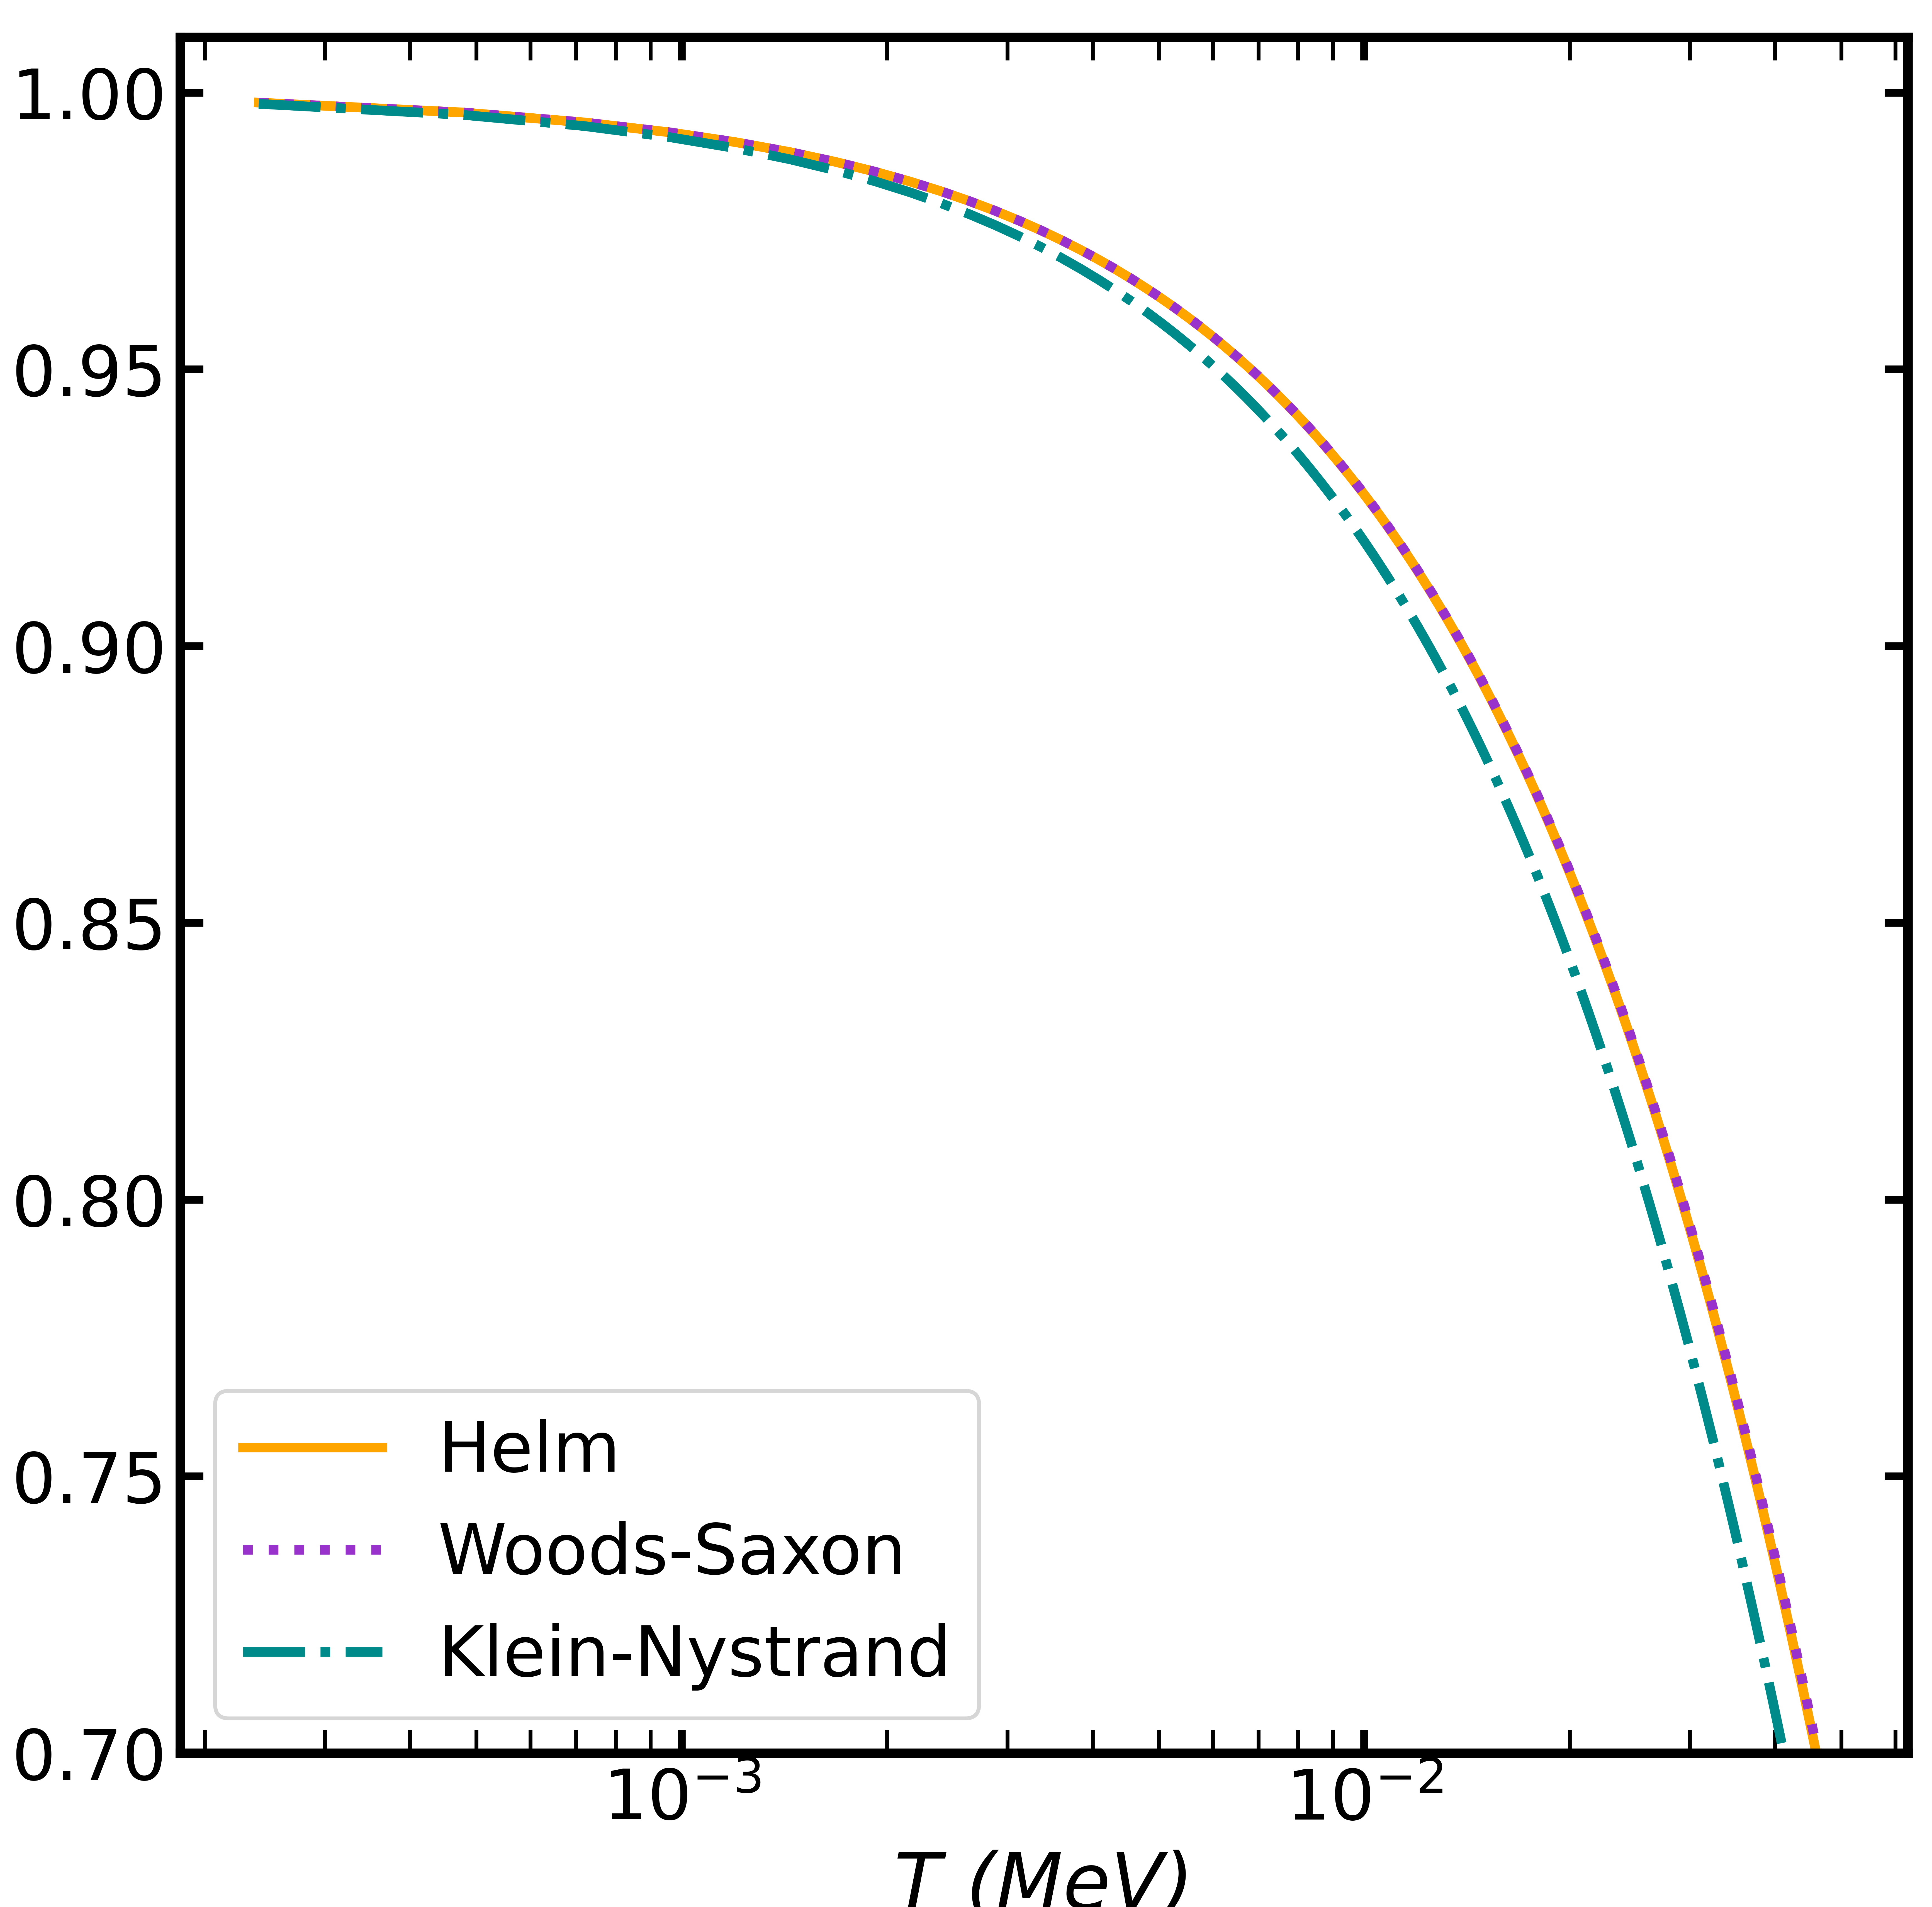
\includegraphics[scale=0.43]{figures/FFC.png}}
     \caption{Nuclear form factor of $^{64}Zn$  compared for different nuclear methods.}
     \label{fig4}
\end{figure}
\\
A form factor equal to one represents an utterly coherent interaction, as it would assume the nucleus to be point-like. Therefore, using the information mentioned above and Equation (1), the differential cross-section was plotted for the isotope $^{64}Zn$ using different form factors and an incident neutrino energy of 50 MeV to compare them with the utterly coherent case. This can be observed in Figure \ref{fig5}.
\begin{figure}[h!]
     \centering
     \subfigure[\emph{For $E_\nu=50$ MeV, comparing  different nuclear methods, and the point-like nucleus case (F=1)}]{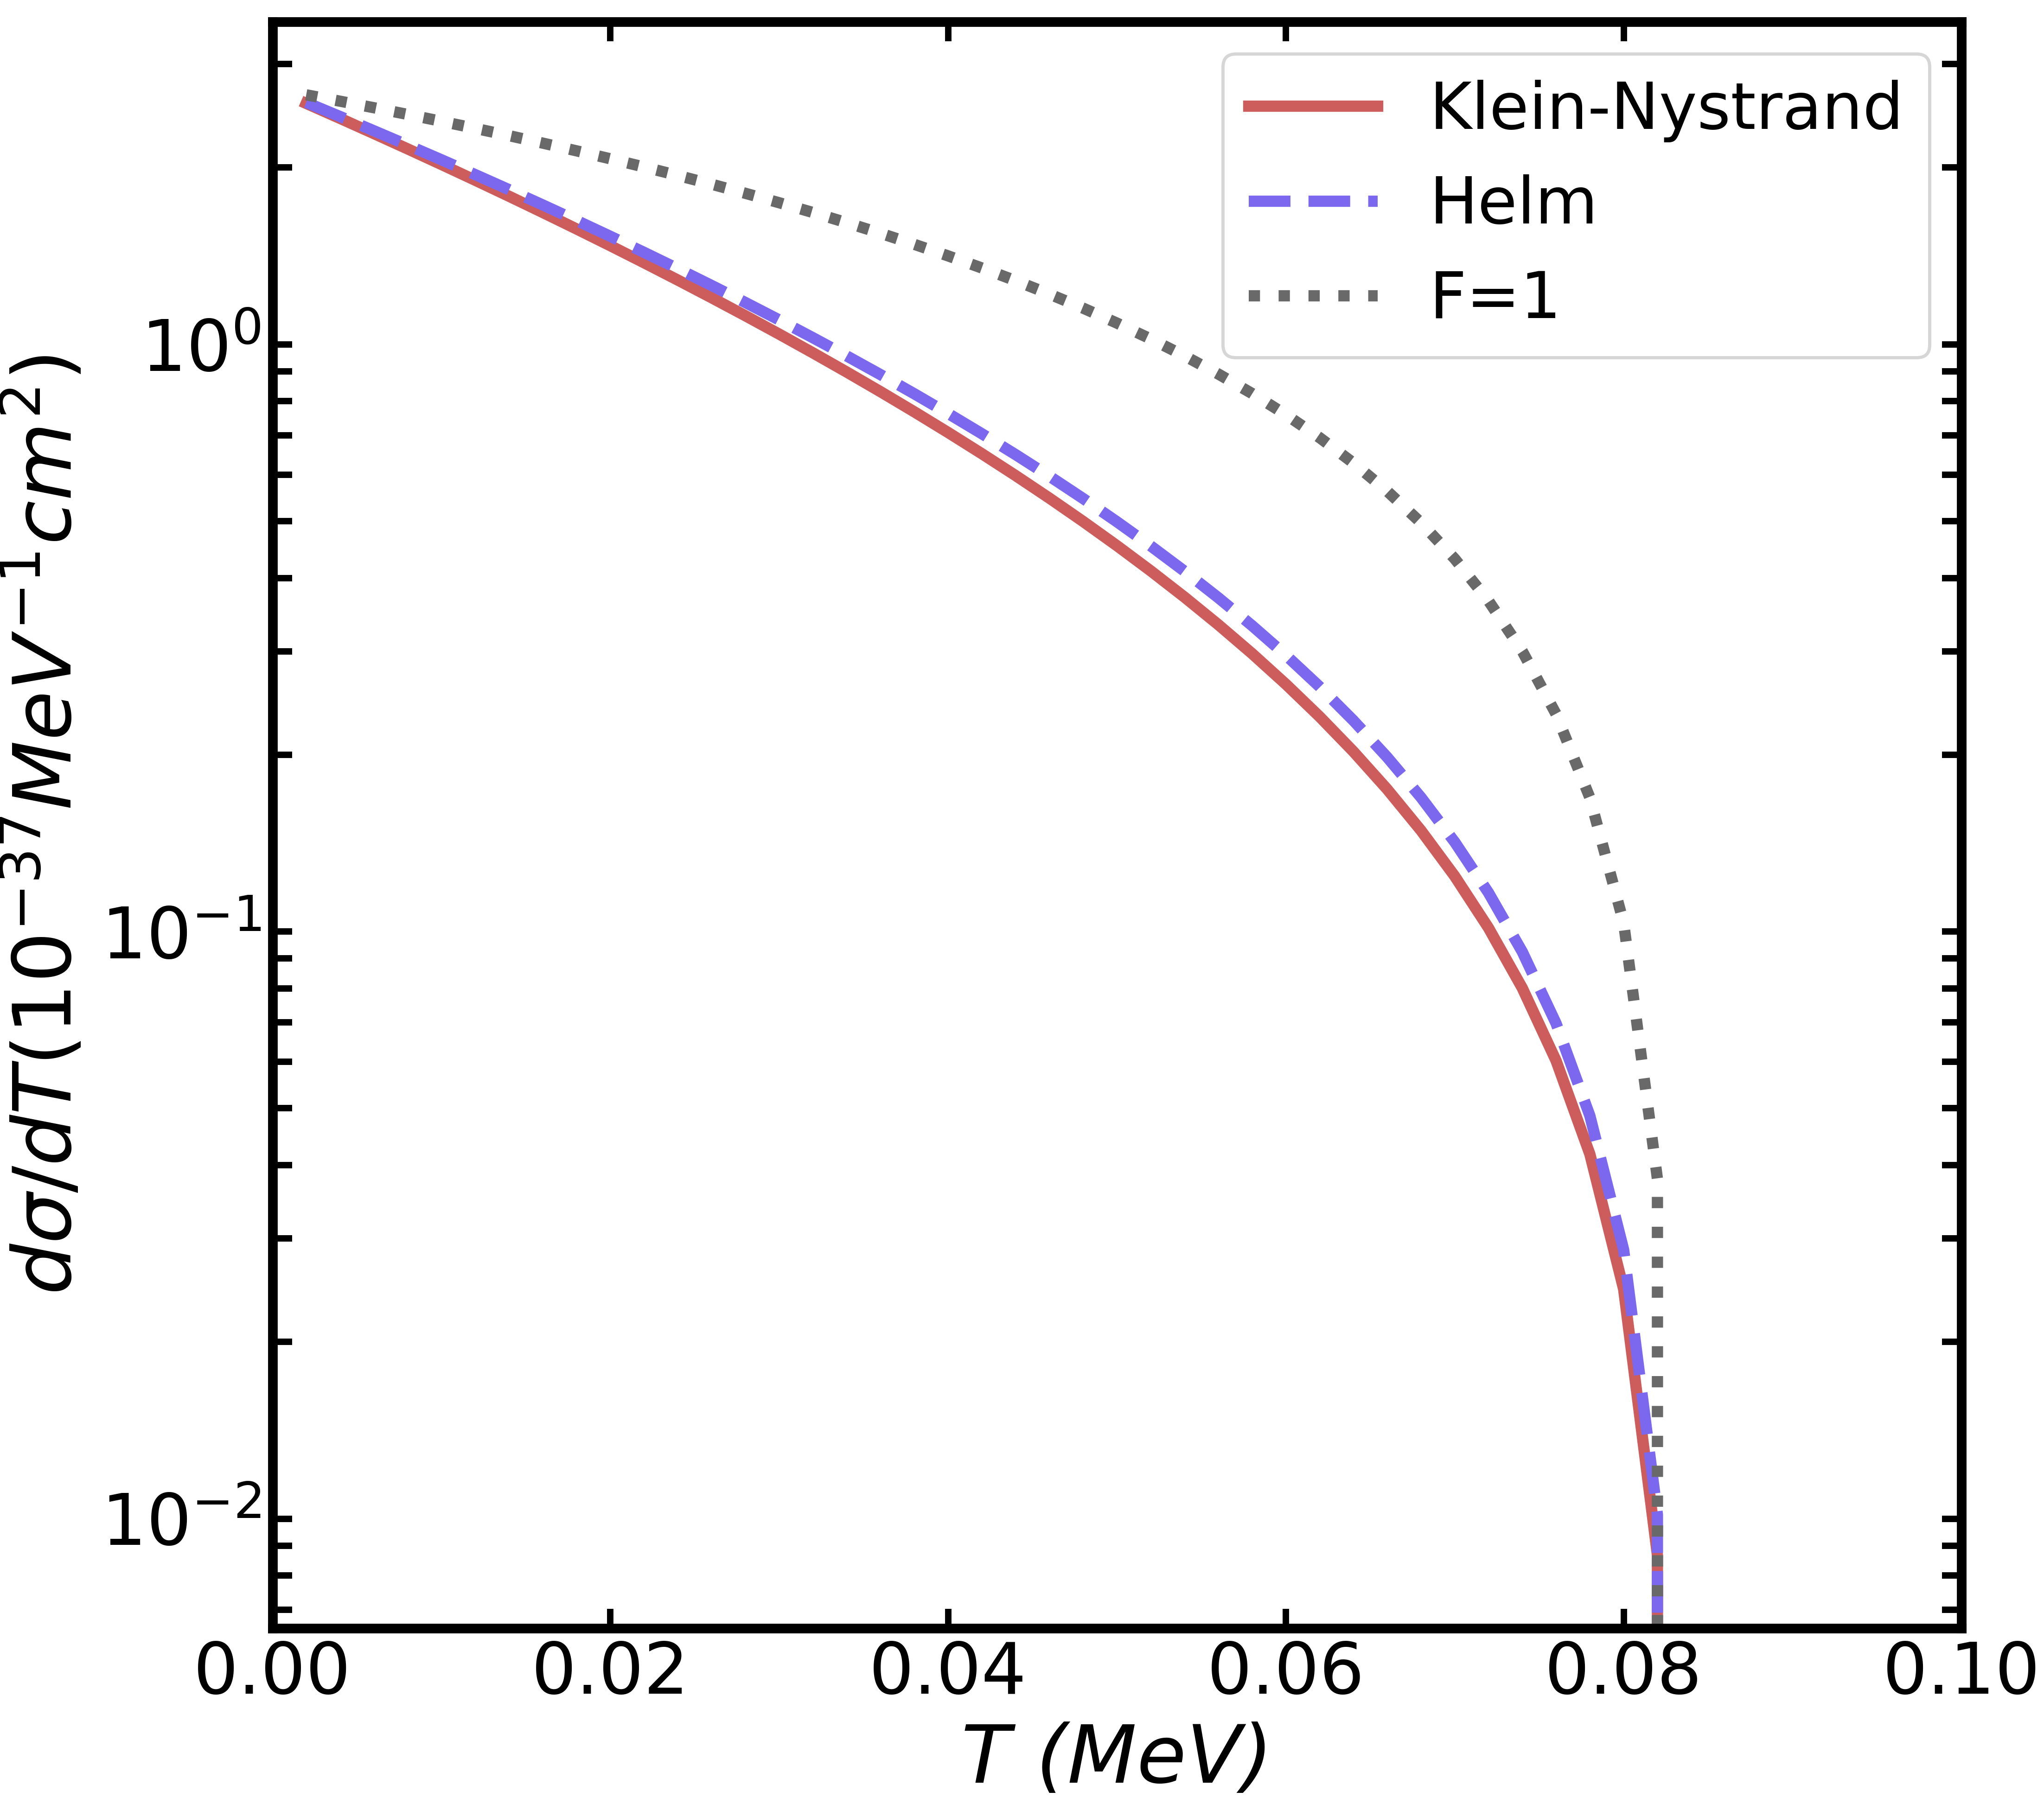
\includegraphics[scale=0.36]{figures/Compara.png}}\hspace{1em}%
     \subfigure[\emph{For different incident neutrino energies. Showing the case of point-like nucleus (F = 1) for $E_\nu$ = 50 MeV and $E_\nu$ = 20 MeV} ]{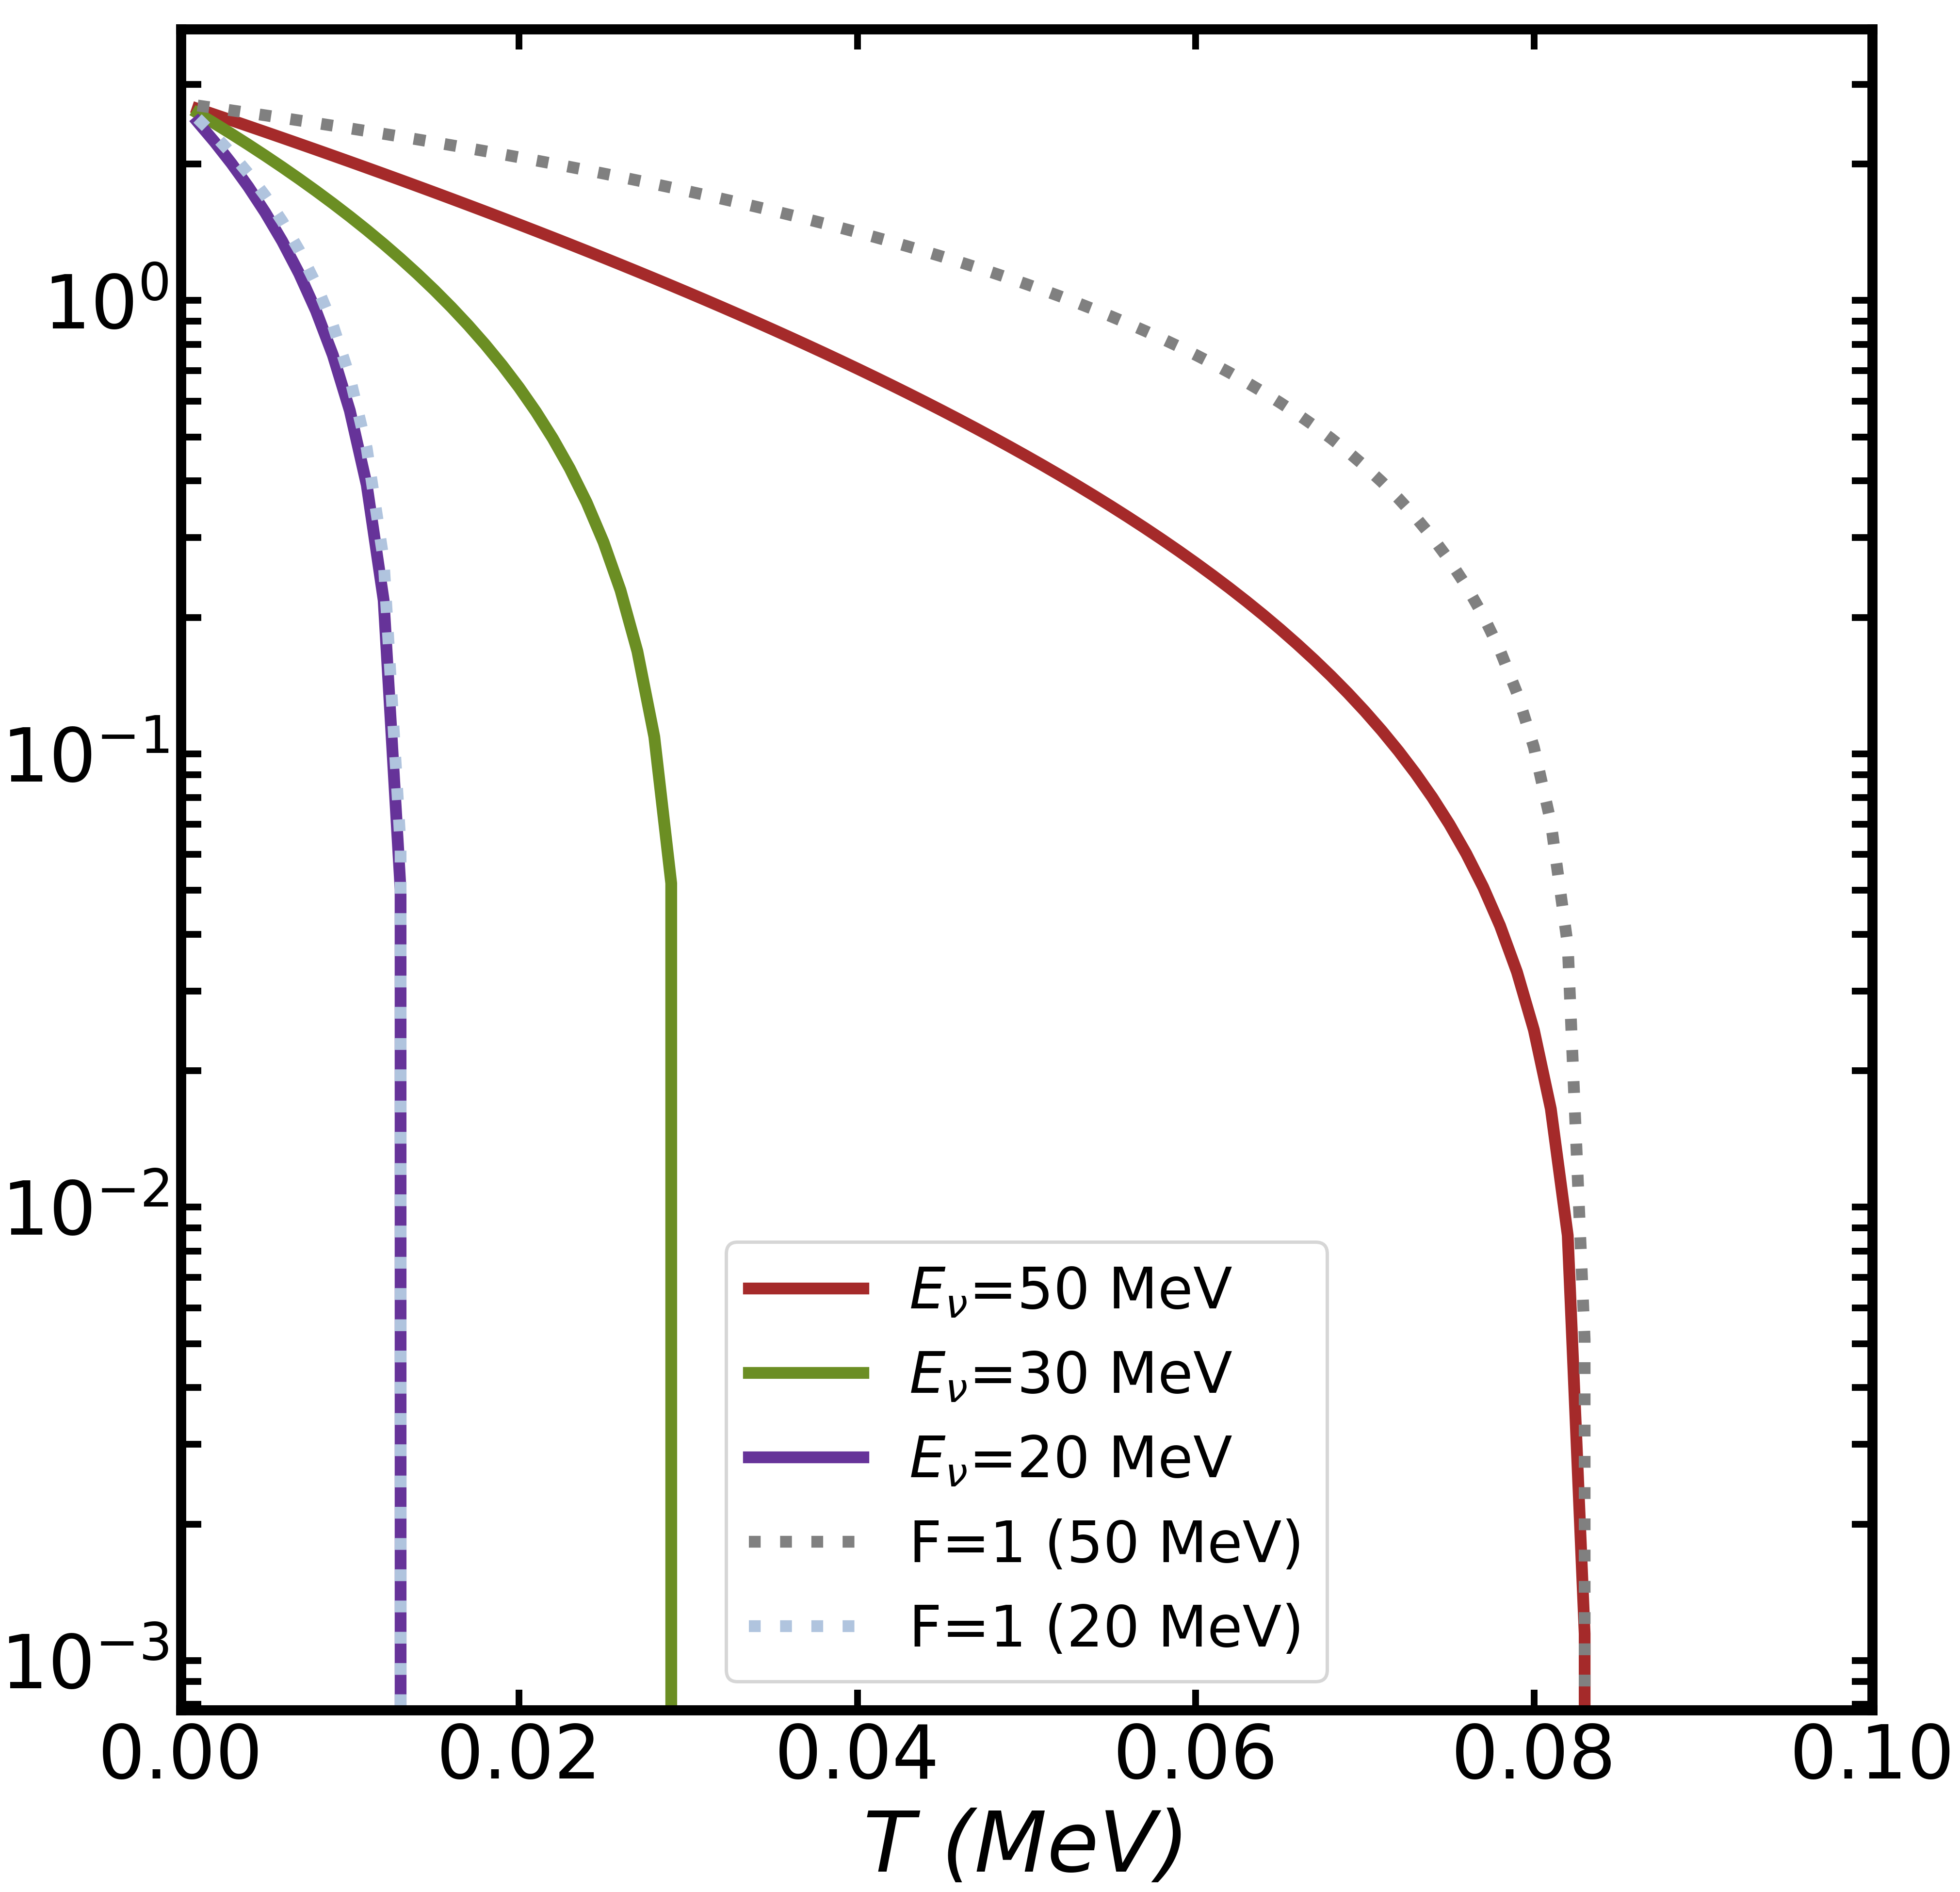
\includegraphics[scale=0.36]{figures/Cross.png}}
     \caption{The differential cross section $d\sigma/dT$ in terms of the nuclear recoil energy T.}
     \label{fig5}
\end{figure}
\section{Neutrino flux}

Many neutrino natural sources could be acceptable for detecting CE$\nu$NS, such as  solar neutrinos,diffuse supernova neutrinos, and low-energy neutrinos from the atmospheric neutrino flux. However, the challenge is that these natural neutrino fluxes are relatively small and would require huge detectors for detection. Therefore, researchers have turned to laboratory-created neutrino beams for their detection purposes.

\subsection{Antineutrinos from reactor}

Nuclear reactors operate through the fission of uranium and plutonium fuel. As part of this process, neutron-rich fission products go through beta decay, which involves the emission of electrons and electron antineutrinos. During beta decay, electrons and antineutrinos are emitted in a continuous energy range with a maximum energy value.  The number of electrons emitted at each energy level constitutes the electron's spectral shape, while its complement describes the antineutrino's spectral shape.

To determine the energy distribution of antineutrinos emitted by nuclear reactors, we combined the spectral shapes of antineutrinos from all beta decays occurring within the reactor. This process allows for obtaining the overall energy distribution of the antineutrinos released by the reactor.

In reactor neutrino experiments, the detection of neutrinos relies on inverse beta decay
\begin{equation*}
    \bar{\nu_e}+p \rightarrow n + e^+.
\end{equation*}
This detection method establishes an energy threshold for the antineutrino at 1.804 MeV, and on the high energy side, antineutrino rates above 8 MeV become negligible \cite{HUBER2016268}.
There are four isotopes whose fission dominates in the production of neutrinos with energy above this inverse decay threshold. These isotopes are $^{235}U$, $^{239}Pu$, $^{241}Pu$, and $^{238}U$. Other isotopes contribute only at a level of 0.1$\%$. However, the resulting flux of neutrinos is a combination of numerous beta-decay branches from the fission fragments of the four isotopes involved.

Reactor neutrino fluxes arising from the thermal fission of $^{235}U$, $^{239}Pu$, and $^{241}Pu$ are determined by analyzing the measured total $\beta$-spectra, obtained at the Institut Laue-Langevin (ILL). Currently, total beta spectra for $^{238}U$ is not available because the isotope undergoes fission exclusively through fast neutrons. As a result, a prediction of the antineutrino spectrum associated with the fission of $^{238}U$ is provided based on an ab initio method, as mentioned in the reference \
\cite{Mueller_2011}.

The inversion process allows researchers to extract the neutrino flux information from these measured spectra. Using these measurements as a basis, a phenomenological parametrization was proposed for the antineutrino flux of the reactor in \cite{PhysRevD.70.053011}.

This parametrization is given by

\begin{equation}
    S(E_\nu)=exp\left(\sum_{p=1}^6 \alpha_{p} E^{p-1}_\nu \right),
\end{equation}


where a data fit determines the coefficients $\alpha_p$. The best coefficients found in the reference \cite{Mueller_2011} are given in table \ref{Coefficients}\\
\vspace{0.7em}


\begin{table}[h]
\centering

 
\begin{tabular}{p{2cm}c c c c}
\toprule
     & $^{235}U$ &   $^{238}U$   & $^{239}Pu$  &  $^{241}Pu$            \\ \midrule
$\alpha_1 $ & 3.217     & $4.833x10^{-1}$ & 6.413 &  3.251                                  \\
$\alpha_2$ &  $-3.111$ & $1.927x10^{-1}$  & $-7.432$ &  $-3.204$         \\
$\alpha_3$ & 1.395 & $-1.283x10^{-1}$ & 3.535 &  1.428   \\
$\alpha_4$   & $-3.690x10^{-1}$     & $-6.762x10^{-3}$  & $-8.820x10^{-1}$ & $-3.675x10^{-1}$  \\
$\alpha_5$ & $4.445x10^{-2}$       &$2.233x10^{-3}$  &   $1.025x10^{-1}$  &   $4.254x10^{-2}$             \\
$\alpha_6$ & $-2.053x10^{-3}$  & $-1.536x10^{-4}$  & $-4.550x10^{-3}$  &$-1.869x10^{-3}$ 
\\
\bottomrule

\end{tabular}
 \caption{Coefficients $\alpha_p$ of the polynomial parametrization \cite{Mueller_2011}}
\label{Coefficients}
\end{table}\\



Figure \ref{flujosReactor} shows the resulting spectra of the parameterization using these coefficients for each of the four main isotopes.
\vspace{0.7em}

\begin{figure}[h!]
    \centering
    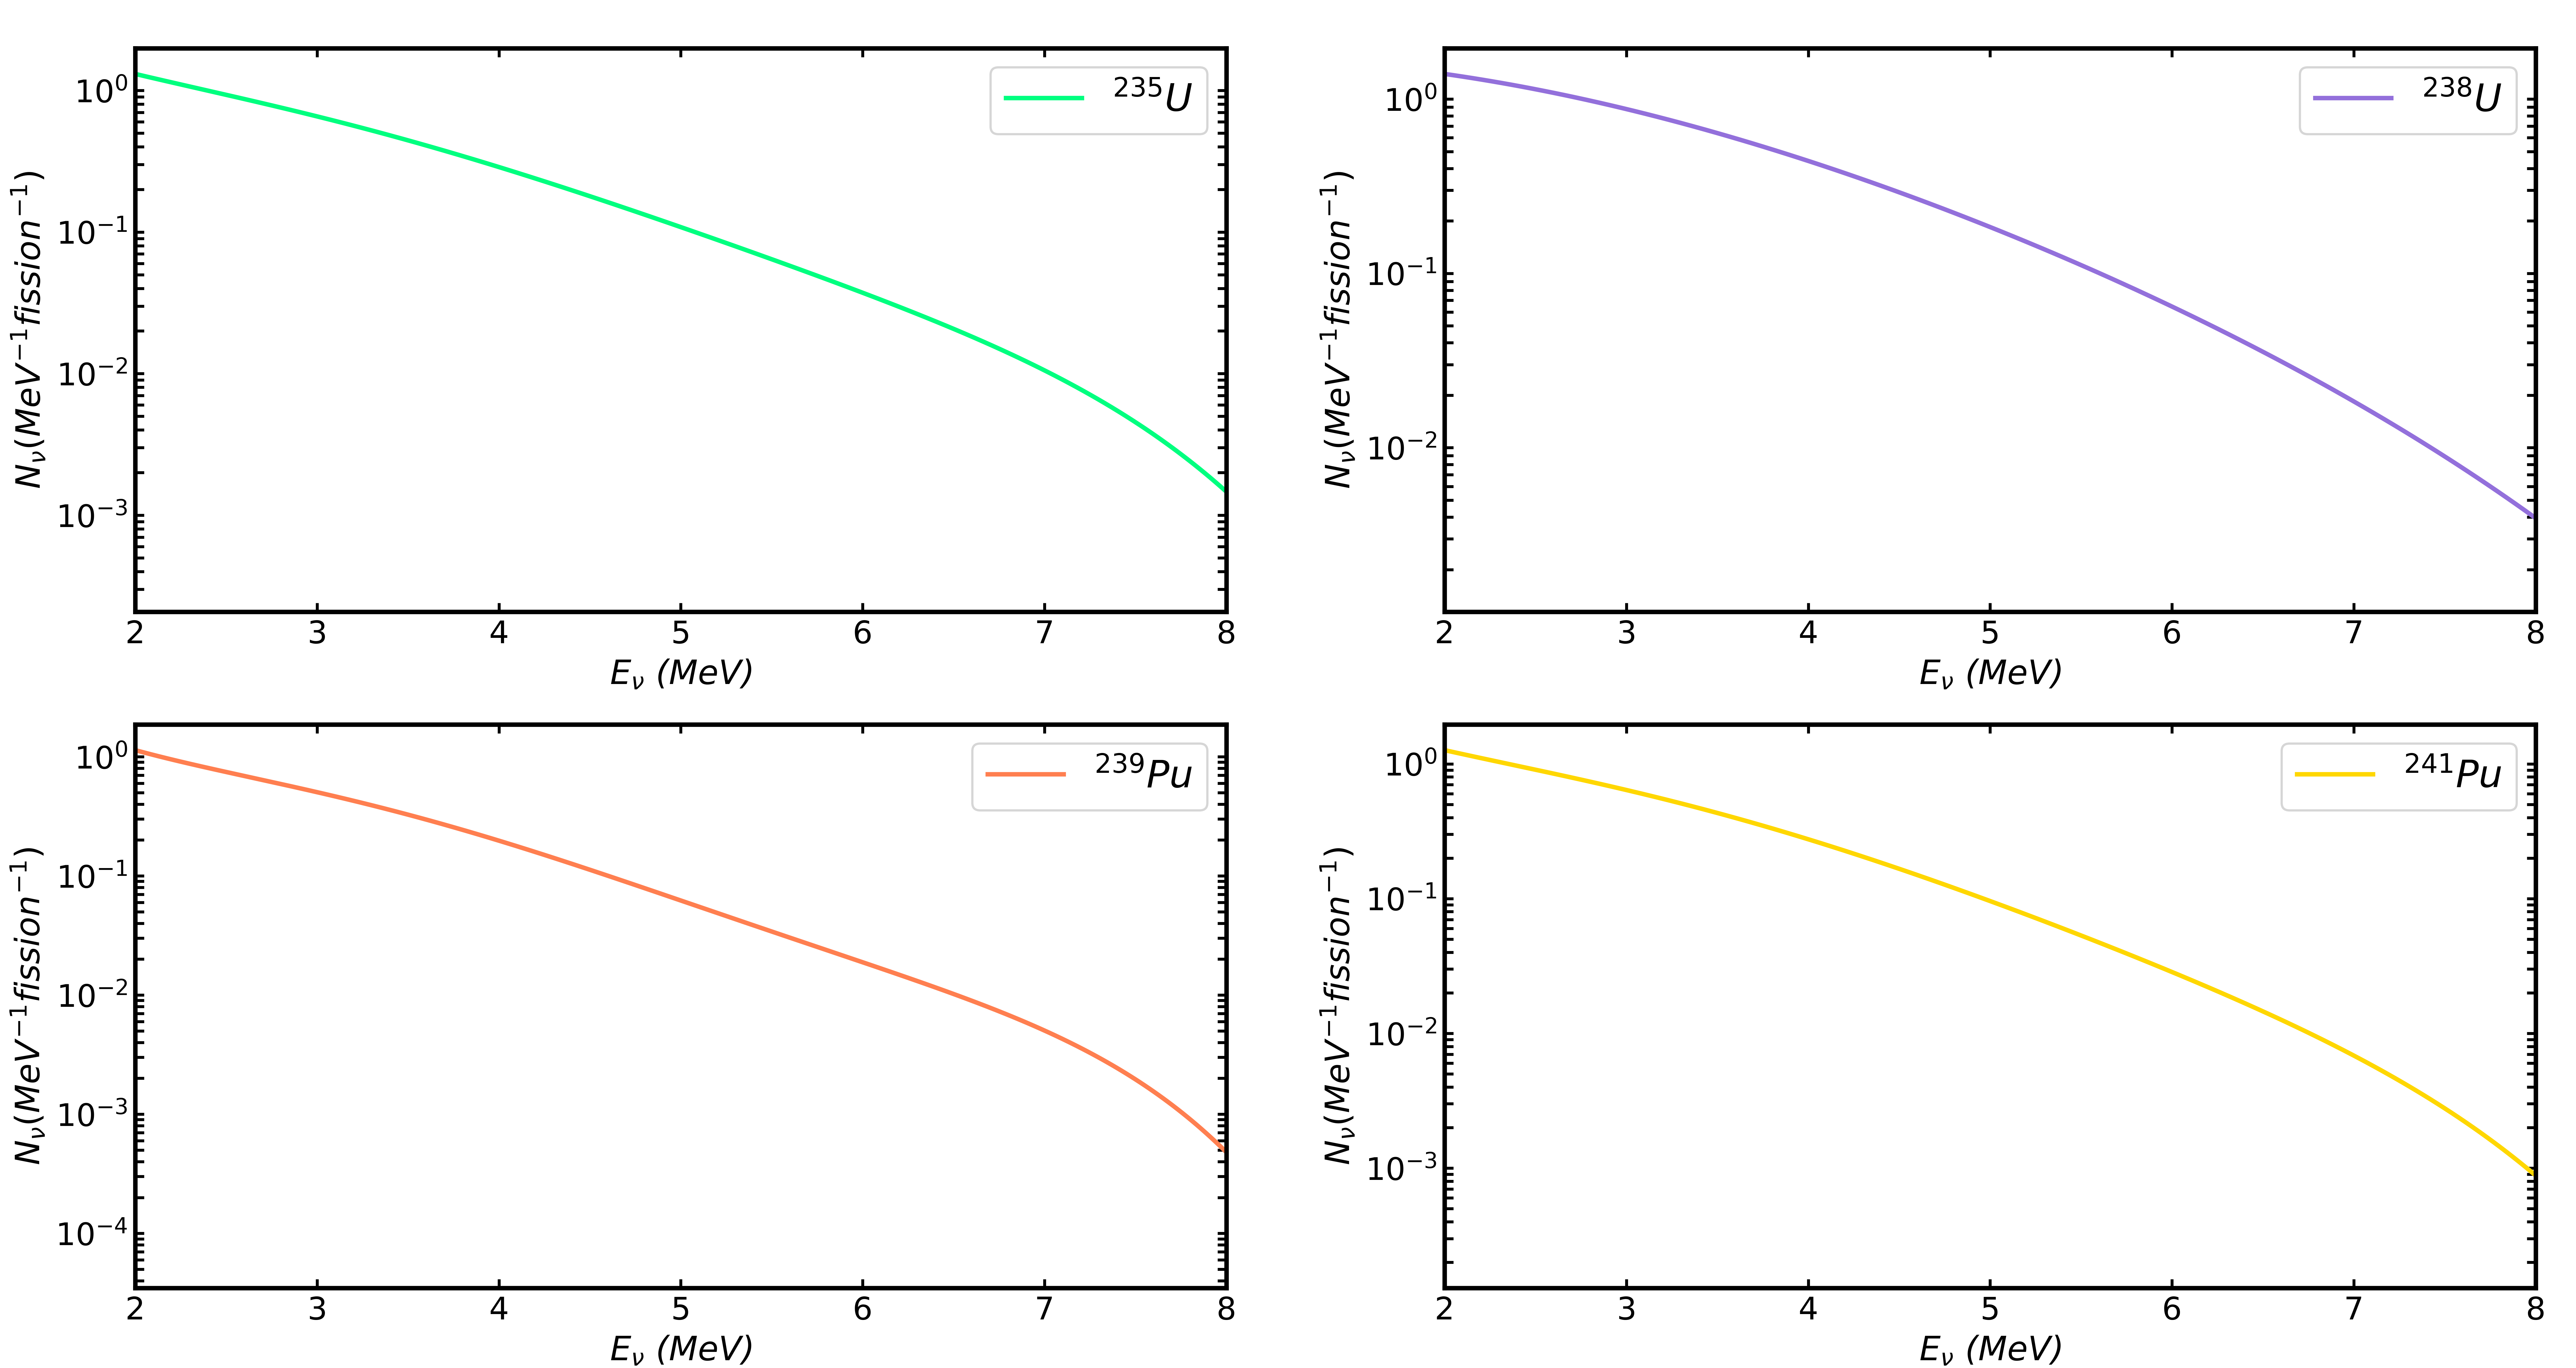
\includegraphics[scale=0.4]{figures/flujosInd.png}
\caption{Antineutrino reactor spectra predicted for each isotope.}
    \label{flujosReactor}
\end{figure}

Considering a fission fraction for isotope $55\%$ of $^{235}U$, $32\%$ of $^{239}Pu$, $7\%$ of $^{238}U$, and $6\%$ of $^{241}Pu$ we obtain a total spectra flux presented in figure \ref{flujostotal}

\begin{figure}[h!]
    \centering
    \includegraphics[scale=0.3]{figures/Total.png}
\caption{Antineutrino reactor total spectra.}
    \label{flujostotal}
\end{figure}

\subsection{Pion Decay At Rest ($\pi$-DAR)}

Reactor neutrinos could be an excellent option for detecting CE$\nu$NS as they produce a large flux of $\bar{\nu_e}$. However, the energy window for reactor neutrinos extends up to approximately 7 MeV, which results in very small nuclear recoils that are difficult to detect. Another option is to use neutrinos generated in accelerator-based reactions. In these cases, high-energy proton beams collide with nuclear targets, producing pions that decay and generate neutrinos. One approach to achieve this is through $\pi$-DAR. This method provides neutrino fluxes at the Spallation Neutron Source, where a prompt component of the $\nu_\mu$ flux is obtained from the decay of pions at rest, along with two delayed components of $\bar{\nu_\mu}$ and $\nu_e$ from the decay of muons produced in the initial decay process \cite{Cadeddu_2018}. These processes are illustrated below.
\\
\begin{equation*}
    \pi^+ \rightarrow \mu^+ + \nu_\mu \qquad \Rrightarrow \qquad \mu^+ \rightarrow e^+ + \bar{\nu}_\mu +\nu_e,
\end{equation*}

their respective fluxes are described by
\\
\begin{equation}
    \frac{dN_{\nu_\mu}}{dE}=\eta\delta \left(E-\frac{m_\pi^2-m_\mu^2}{2m_\pi}\right),  
\end{equation}
\begin{align}
    \frac{dN_{\bar{\nu_\mu}}}{dE}=\eta \frac{64E^2}{m_\mu^3}\left(\frac{3}{4}-\frac{E}{m_\mu}\right),
\end{align}
\begin{align}
    \frac{dN_{\nu_e}}{dE}=\eta \frac{192E^2}{m_\mu^3}\left(\frac{1}{2}-\frac{E}{m_\mu}\right).
\end{align}
\\
The total flux $dN_\nu/dE$ will be the sum of these three fluxes. $\eta$ is the normalization constant $\eta = rN_{\text{POT}}/(4\pi L^2)$, which incorporates parameters related to both the neutrino flux and detector. Here, $r$ represents the number of target nuclei in the detector, $N_{\text{POT}}$ is the number of protons on target (POT), and $L$ denotes the distance between neutrino source and detector.
\begin{figure}[h!]
    \centering
    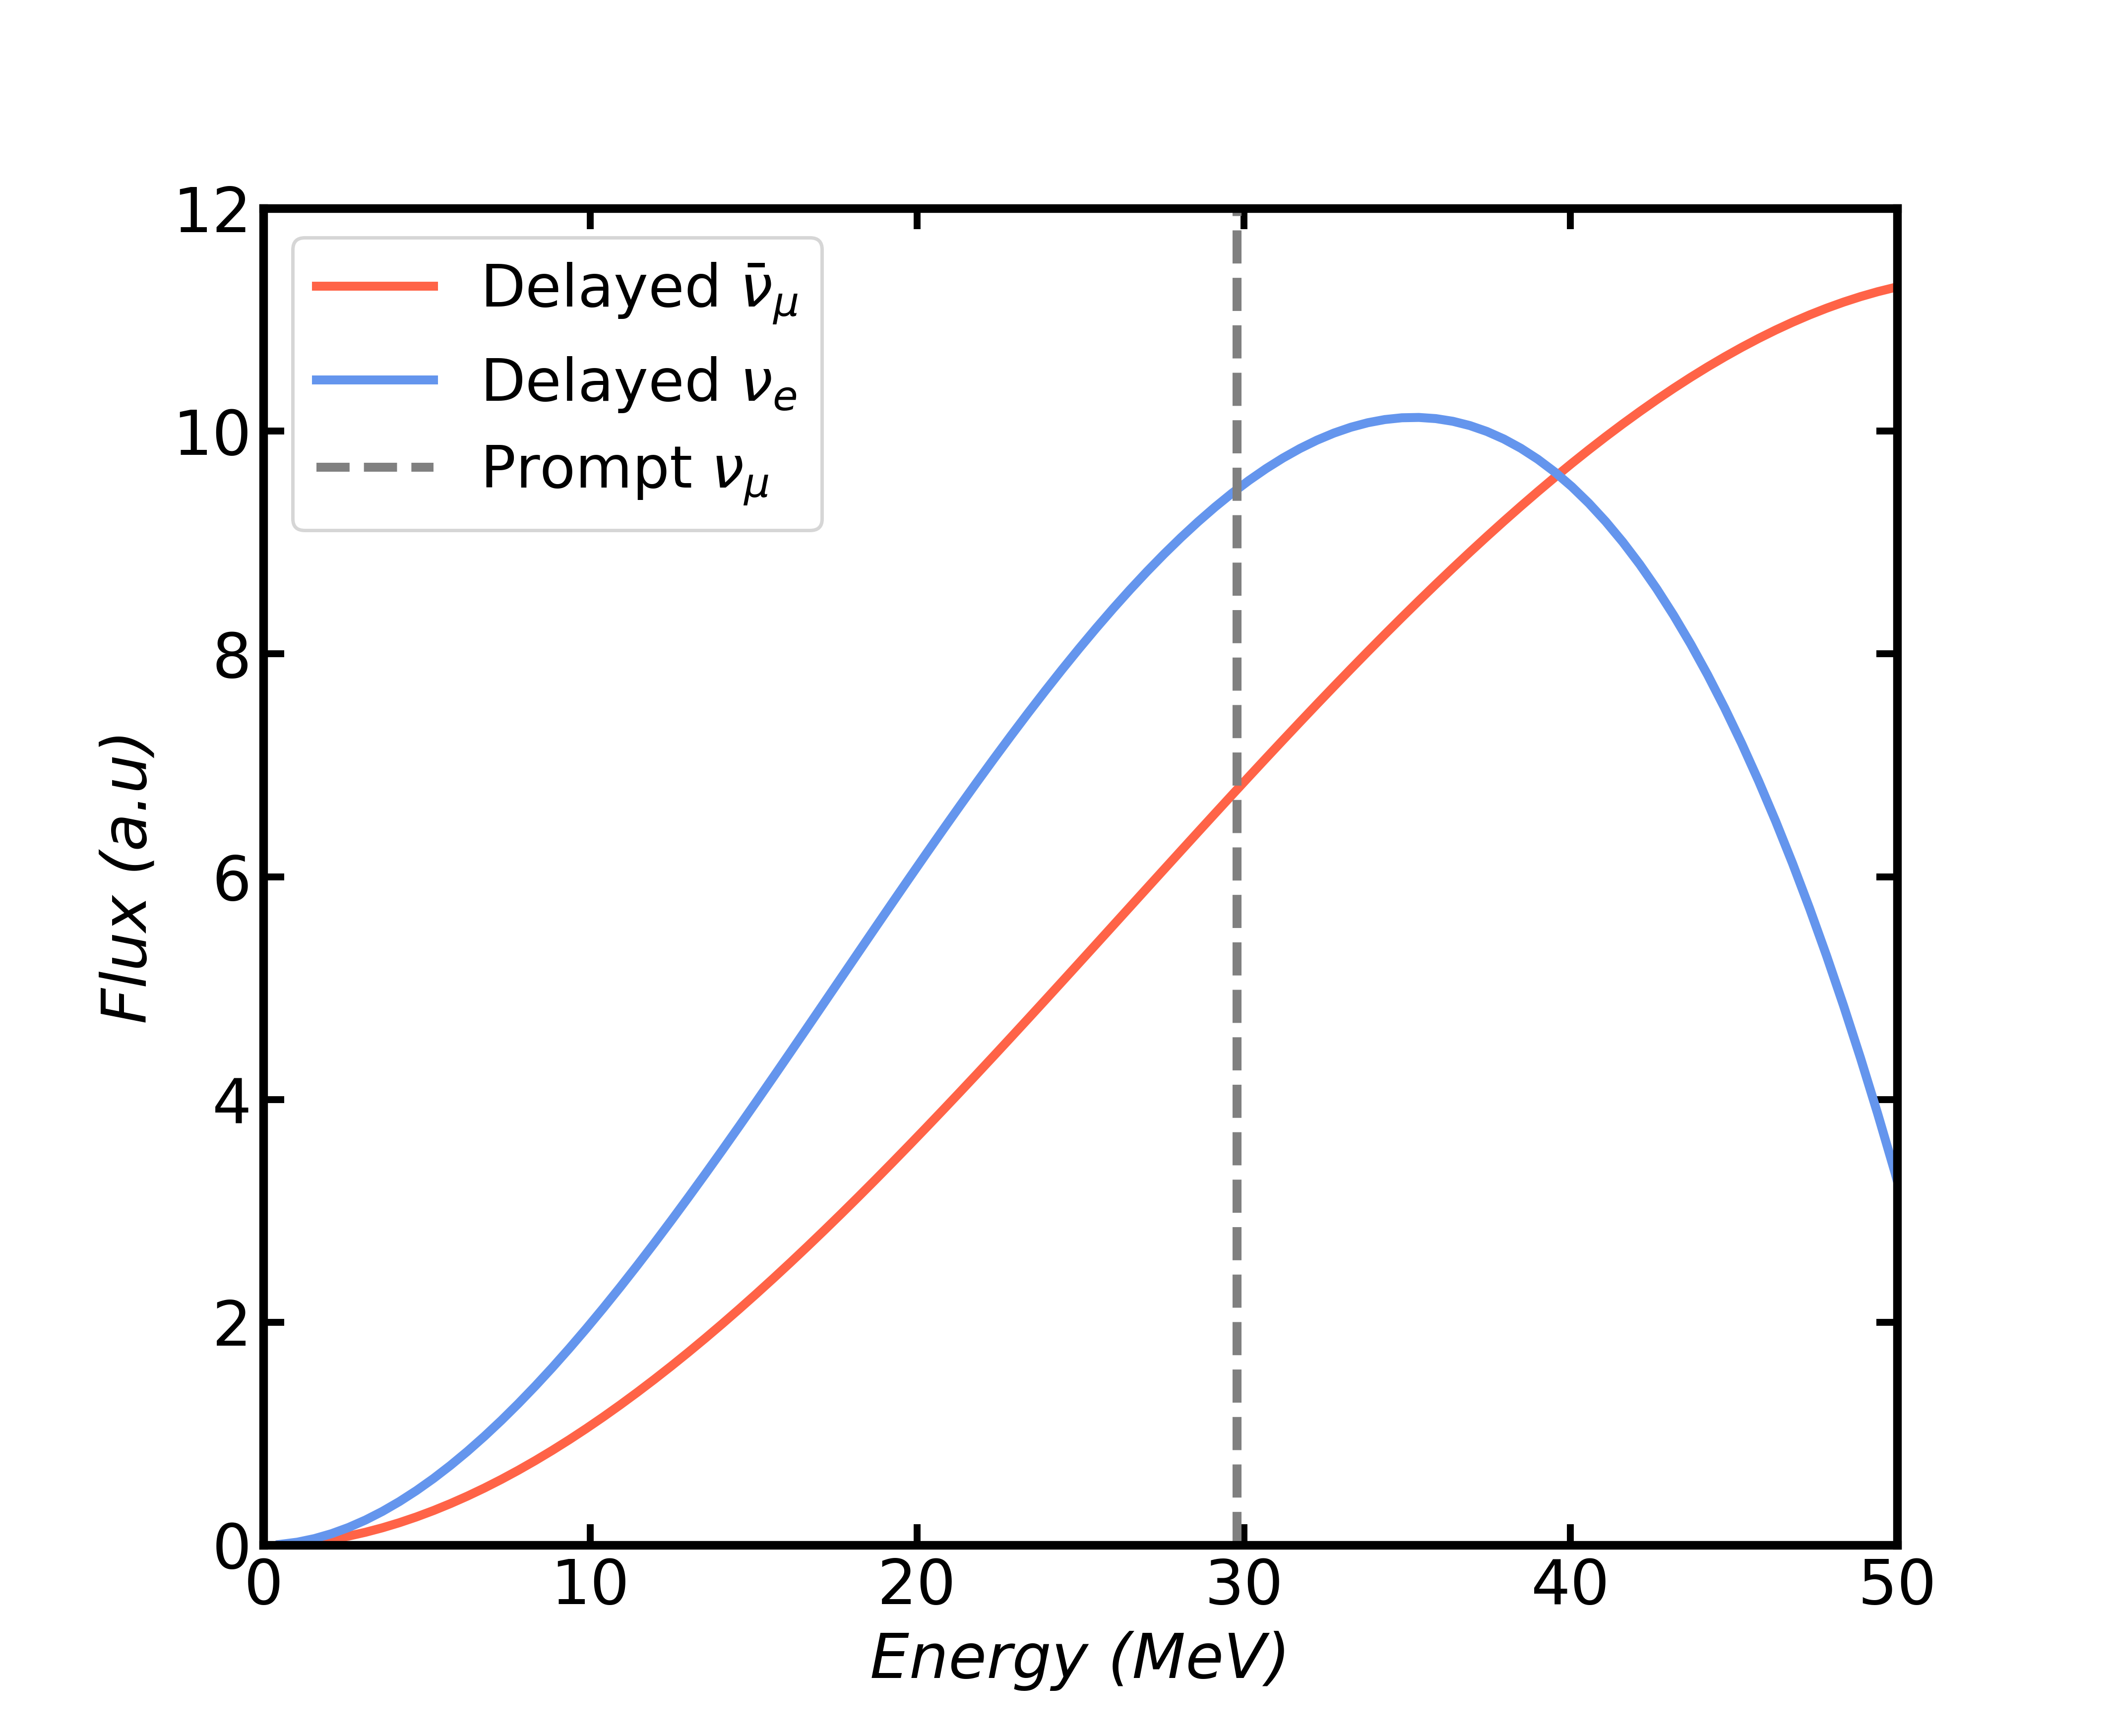
\includegraphics[scale=0.5]{figures/Flux.png}
\caption{Neutrinos flux at SNS}
    \label{fig7}
\end{figure}

\section{Events}
By the number of events, we refer to the number of neutrino interactions with the target (detector). The expected number of neutrino events is proportional to the neutrino flux, the cross-section, and the number of targets in the detector:
\\
\begin{equation*}
    N_\nu(E)\propto \phi_\nu(E) \sigma_\nu(E) N_{Target}.
\end{equation*}
Therefore, the differential event rate is given by
\\
\begin{equation}
    \frac{dR}{dT}=t_{run}N_{targ}\int_{E_{\nu,min}}^{E_{\nu,max}} \frac{d\sigma}{dT}\frac{dN\nu}{dE}\,dE.
\end{equation}
\\
The running time is denoted as $t_{run}$. $N_{targ}$ is the number of atoms in the detector, which is calculated as $N_a M_{det}/M_D$, where $N_a$ is Avogadro's number and $M_D$ is the molar mass. The lower limit of the integral with respect to E is obtained from kinematics and is given by \cite{kosmas}
\\
\begin{equation}
    E_{\nu,min}= \frac{1}{2}\left( T^2+\sqrt{T^2+2MT}\right) \approx \sqrt{\frac{MT}{2}}.
\end{equation}
\\
This integral's upper limit depends on the produced neutrinos' maximum energy. For those produced by $\pi$-decay at rest ($\pi$-DAR), it will be $E_{\nu,max}=m_{\mu}/2=52.8 MeV$. A second integration with respect to the recoil energy of the nucleus is performed to obtain the total number of events. The lower limit of this integral depends on the detector threshold and the upper limit depends on the maximum recoil energy given by kinematics
\\
\begin{equation}
    T_{max}=\frac{2 E_{\nu,max}^2}{2 E_{\nu,max}+M} \approx \frac{2 E_{\nu,max}^2}{M}.
\end{equation}

The pull method is utilized to compare theoretical expectations with experimental data. The parameter bounds can be set at a desired confidence level by minimizing a least squares function, $\chi^2$, as presented in the following chapter.
\section{CE$\nu$NS experiments}

As previously mentioned, CE$\nu$NS was proposed in 1974, leading to various experiments conducted over the years. In 1984, a technique for detecting neutrinos using CE$\nu$NS interactions via superconducting grains was put forth by Drukier and Stodolsky \cite{Drukier}. This method employs superconducting grains, in a metastable state within a dielectric material located within a magnetic field.\\

Subsequently, various types of detectors were proposed to address this challenge. In 2000, McKinsey and Doyle \cite{mckinsey1999liquid}, followed by Horowitz in 2003 \cite{Horowitz}, introduced a neutrino detection approach utilizing scintillation in noble gases. This method, known as the CLEAN (Cryogenic Low Energy Astrophysics with Noble gases) detector, relies on the weak ionization signal generated by nuclear recoil in the liquid. In 2004, Hagmann and Bernstein proposed applying the same principle to a two-phase argon ionization detector \cite{Hagmann_2004}.\\
 Another approach, suggested by Oberauer in 2002 \cite{OBERAUER2002301}, involves cryogenic detectors, similar to those developed for dark matter searches, for neutrino detection. The main idea in this case would to measure the phonons by using low-temperature calorimeters.\\
In 2006, Scholberg analyzed advancements in ultra-low-threshold detector technology in recent years. Proposed detectors include noble element scintillation detectors, ionization detectors, solid-state detectors, bubble detectors, and superheated droplet detectors \cite{Scholberg}.

Currently,  numerous experiments are dedicated to detecting CE$\nu$NS, with notable examples including the COHERENT Collaboration, among others.


\subsection{COHERENT}

Formed in 2014, the COHERENT Collaboration operates from the Spallation Neutron Source (SNS) situated in the Oak Ridge National Laboratory. The SNS serves as a pulsed neutron source, generating a notable quantity of pulsed neutrinos through stopped-pion decay. It is capable of producing around $8 \times 10^4$ neutrinos per flavor per second as a result of the 1 GeV proton beam incident on a liquid mercury target.

\begin{figure}[h!]
    \centering
    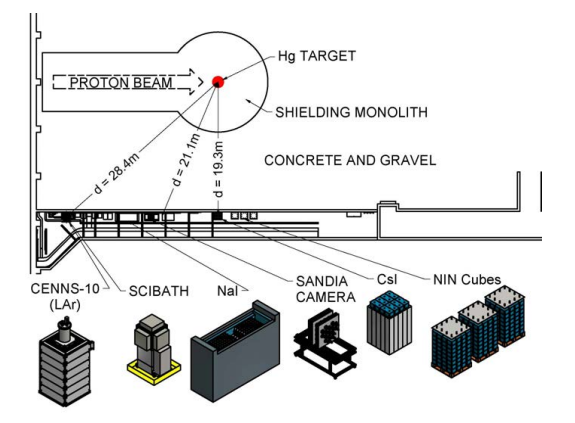
\includegraphics[scale=1.2]{figures/Coherent.png}
    \caption{Schematic representation of the COHERENT experiment. \cite{Akimov_2017}}
    \label{Coherent}
\end{figure}

The COHERENT Collaboration is actively engaged in deploying diverse components or modules, utilizing a range of target nuclei and detector technologies to observe neutrinos originating from the SNS. This facility is positioned in a region known as "Neutrino Alley," situated at a distance of 19-29 meters from the mercury target, as illustrated in Figure \ref{Coherent}.


In 2017, the Collaboration detected Coherent Elastic Neutrino-Nucleus Scattering (CEvNS) utilizing a 14.6 kg CsI[Na] detector, employing the "scintillation detection" method. This technique involves using a target material, in this case, cesium iodide (CsI), comprised of low-energy threshold nuclei capable of efficient interaction with neutrinos. Notably, they achieved the first measurement of CEvNS on argon in 2020, as reported in \cite{akimov2022coherent}.

\subsection{Ricochet}

The Ricochet experiment aims to detect Coherent Elastic Neutrino-Nucleus Scattering (CE$\nu$NS) utilizing the neutrino flux from the reactor at ILL (Institut Laue-Langevin) in Grenoble, France. Two proposed detectors for this experiment include Crycub, composed of 27 high-purity germanium crystal detectors with a total mass of approximately one kilogram. These detectors, enclosed in a radio-pure copper box suspended below inner shielding, aim to minimize background noise. The Q-array, another detector within Ricochet, consists of nine cubes made of superconducting zinc. This use of superconductors introduces innovative technology with a theoretical detection threshold at the Cooper pair binding energy, enhancing sensitivity to extremely low-energy interactions. The incorporation of superconducting zinc cubes in the Q-array holds promise for increasing the sensitivity, precision, and accuracy of the Ricochet experiment \cite{ricochetcollaboration2021ricochet}.

\subsection{CONNIE}

Established in 2014, CONNIE (COherent Neutrino-Nucleus Interaction Experiment) is situated in close proximity to the core of the 3.8 GW Angra 2 nuclear reactor in Rio de Janeiro, Brazil, approximately 30 meters away. Housed within a laboratory set up in a shipping container at sea level just outside the reactor dome, the experiment benefits from an estimated neutrino flux density of around $7.8\times10^{12}\bar{\nu}s^{-1}cm^{-2}$ \cite{Nasteva_2021}. CONNIE's primary objective is to detect the coherent scattering of antineutrinos from silicon nuclei, achieved through the use of fully depleted high-resistivity CCDs (Charged Coupled Devices). CCDs, silicon-based sensors with low noise and threshold levels, are deemed excellent for detecting low-energy depositions, especially those resulting from the coherent scattering of neutrinos off nuclei \cite{Fernandez_Moroni_2015}.

\subsection{CONUS}

The CONUS (COherent Neutrino nUcleus Scattering) experiment is dedicated to investigating coherent elastic neutrino-nucleus scattering of reactor antineutrinos at the Brokdorf commercial nuclear power plant (KBR) in Germany. The experimental setup includes four p-type point contact high-purity germanium (HPGe) detectors, with each cylindrical germanium (Ge) diode weighing approximately 0.996 kg. Positioned just 17.1 meters from the reactor core center, these detectors experience an antineutrino flux of about $2.3\times10^{13}s^{-1}cm^{-2}$ when the reactor operates at its maximum thermal power of 3.9 GW \cite{Bonet_2021}.\\
The CONUS experiment, utilizing germanium detectors, has not only contributed to the search for coherent elastic neutrino-nucleus scattering but has also imposed initial constraints on the electromagnetic properties of neutrinos, particularly through neutrino-electron scattering. Notably, it has set upper limits for the effective neutrino magnetic moment and the effective neutrino millicharge based on the data acquired from the experiment \cite{Elect}.  

\subsection{MINER}

The primary objective of MINER (Mitchell Institute Neutrino Experiment at Reactor) is to precisely measure the Coherent Elastic Neutrino-Nucleus Scattering (CE$\nu$NS) cross-section, utilizing a substantial neutrino flux of approximately $10^{17}$ neutrinos per second from the 1 MW reactor \cite{Miner}. The experiment employs two types of low-energy thresholds: phonon-mediated cryogenic silicon detectors. One of these detectors offers single electron sensitivity, while the other allows for event-by-event signal discrimination from background noise. Moreover, the distance between the reactor core and the detector is adjustable, ranging from 1 to 10 meters. This flexibility enables the observation of short baseline neutrino oscillations and enhances the understanding of background sources.

\subsection{ CAPTAIN-Mills}

The Coherent CAPTAIN-Mills (CCM) detector is positioned at the Los Alamos Neutron Science Center within the Los Alamos National Laboratory. Weighing 10 tons, this detector utilizes liquid argon (LAr) as the detection medium and is located 20 meters from a high-flux neutron/neutrino source. The CCM experiment leverages abundant pion production to explore dark matter originating from $\pi^0$ decay and to measure mono-energetic 30 MeV muon-neutrinos resulting from $\pi^+$ decay \cite{aguilararevalo2022dark}. The primary goals of the CCM experiment include the search for sterile neutrinos and the investigation of light-dark matter (LDM).
 \newpage
\section{Applications}

The investigation of coherent elastic neutrino-nucleus scattering (CE$\nu$NS) events serves as a valuable tool for exploring physics within the Standard Model as well as beyond it.\\
Indeed, coherent elastic neutrino-nucleus scattering provides a unique opportunity to access the neutron form factor directly and, consequently, the nucleon density within atomic nuclei. As CE$\nu$NS is primarily sensitive to the weak form factor, which is predominantly determined by the coupling to neutrons, this process enables the investigation of neutron distribution within nuclei \cite{Coloma_2020}. The COHERENT experiment provided valuable data that allowed for the first-ever determination of the average radius (rms) of neutrons in Cs and I. Obtaining a value of $R_n=5.5^{+0.9}_{-1.1} $ fm using the symmetrized Fermi and Helm form factors \cite{Cadeddu_2018}.\\
Furthermore, the study of coherent elastic neutrino-nucleus scattering will not only enhance precision tests of the Standard Model but also provide greater sensitivity to the electromagnetic properties of neutrinos. This includes measurements of the neutrino magnetic moment and the neutrino charge radius \cite{Kosmas_2015}. With data from the CENNS-10 experiment, which detected CEvNS in liquid argon (LAr), it was possible to update the constraints on the electromagnetic properties of neutrinos. In \cite{Miranda_2020}, the following constraints were obtained for the magnetic moments of neutrinos $(\mu_{\nu_e},\mu_{\nu_\mu},\mu_{\bar{\nu_\mu}})< (94,53,78) 10^{-10} \mu_B$  at a 90\% confidence level. They also found restrictions for the neutrino charge radius at $90\%$ C.L\\
\begin{equation*}
\begin{split}
&\left<r^2_{\nu_e}\right> = (-64,-41) \; \text{and} \;(-7,16),\\
&\left<r^2_{\nu_\mu}\right> = (-69,-37) \; \text{and} \;(-10,21),\\
&\left<r^2_{\bar{\nu_\mu}}\right> = (-60,-43) \; \text{and} \;(-5,12).
\end{split}
\end{equation*}
In units of $10^{-32} cm^2$.

Coherent neutrino-nucleus scattering is a powerful tool for investigating active to sterile neutrino oscillations \cite{Anderson_2012}. This experimental approach has the potential to confirm the definitive presence of sterile neutrinos and determine precise constraints on their mixing parameters. \\
The knowledge acquired through advancements in new detector technologies holds significant relevance for astrophysics and cosmology \cite{Drukier}. Specifically,  CE$\nu$NS is expected to play a crucial role in various astrophysical phenomena. For example, in the context of supernovae, CE$\nu$NS contributes to the cooling and heating processes that occur during the stellar collapse. Furthermore, CE$\nu$NS interactions involving solar, diffuse supernova remnants, and atmospheric neutrinos occur in dark-matter detectors and produce an irreducible background known as the "neutrino floor". Precisely measuring the CE$\nu$NS cross-section enables better predictions of this background, thus improving our understanding and modeling of astrophysical observations. 

In conclusion, this research has significant implications for our understanding of neutrino physics. It may open up new avenues for exploring the fundamental nature of neutrinos and the underlying principles of particle physics.



